% wirtschaftswunder_1960_1973.tex
\chapter{Das Wirtschaftswunder (1960–1973)}
\label{chap:wirtschaftswunder}

\section*{Einleitung}
Die Phase von 1960 bis 1973 markiert die Hochzeit des deutschen „Wirtschaftswunders“ – eine Periode beispiellosen wirtschaftlichen Aufschwungs bei gleichzeitiger sozialer Spannungen. Dieser Abschnitt analysiert die Entwicklung des GWI-D während dieser Ära und deckt die \textbf{Diskrepanz zwischen ökonomischem Boom und sozialer Stagnation} auf.

\section{Kontext und historischer Hintergrund}

Die Nachkriegsära war geprägt von:
\begin{itemize}
    \item \textbf{Rekordwachstum}: Durchschnittliches BIP-Wachstum von 4,8\% pro Jahr
    \item \textbf{Vollbeschäftigung}: Arbeitslosenquote sank unter 1\% 
    \item \textbf{Technologischer Aufbruch}: Automatisierung, beginnende Computerisierung
    \item \textbf{Soziale Unruhen}: Studentenbewegung 1968, wachsende Ungleichheit
\end{itemize}

Die „Soziale Marktwirtschaft“ Ludwig Erhards schuf einen Rahmen, der wirtschaftliche Freiheit mit sozialem Ausgleich zu verbinden suchte – ein Konzept, dessen Umsetzung in der Praxis jedoch Lücken aufwies.

\begin{table}[ht]
    \centering
    \caption{Makroökonomische Kennzahlen Deutschland 1960–1973}
    \label{tab:makro_wirtschaftswunder}
    \begin{tabular}{lcccc}
        \toprule
        \textbf{Jahr} & \textbf{BIP-Wachstum (\%)} & \textbf{Inflationsrate (\%)} & \textbf{Arbeitslosenquote (\%)} & \textbf{Lohnquote (\%)} \\
        \midrule
        1960 & 8.8 & 1.5 & 1.3 & 65.2 \\
        1963 & 3.5 & 2.8 & 0.8 & 66.1 \\
        1966 & 2.8 & 3.5 & 0.7 & 66.8 \\
        1969 & 7.5 & 1.9 & 0.8 & 68.2 \\
        1972 & 4.2 & 5.5 & 1.1 & 70.1 \\
        1973 & 4.9 & 6.9 & 1.2 & 71.3 \\
        \midrule
        \textbf{Durchschnitt} & \textbf{5.4} & \textbf{3.7} & \textbf{0.9} & \textbf{67.9} \\
        \bottomrule
    \end{tabular}
\end{table}

\begin{flushleft}
\footnotesize{\textit{Quelle: Statistisches Bundesamt, Sachverständigenrat. Lohnquote = Anteil der Arbeitnehmerentgelte am Volkseinkommen.}}
\end{flushleft}

\section{Entwicklung der GWI-D Komponenten}

\begin{table}[ht]
    \centering
    \caption{GWI-D Komponenten während des Wirtschaftswunders}
    \label{tab:gwi_wirtschaftswunder}
    \begin{tabular}{lccccc}
        \toprule
        \textbf{Jahr} & \textbf{W (\(W\))} & \textbf{G (\(G\))} & \textbf{Z (\(Z\))} & \textbf{S (\(S\))} & \textbf{GWI-D Gesamt} \\
        \midrule
        1960 & 76.2 & 60.8 & 65.4 & 70.1 & 69.2 \\
        1963 & 79.5 & 62.1 & 67.2 & 71.8 & 71.4 \\
        1966 & 81.8 & 63.5 & 68.9 & 73.4 & 73.1 \\
        1969 & 85.3 & 65.2 & 71.8 & 75.6 & 76.2 \\
        1972 & 87.6 & 66.8 & 73.5 & 77.2 & 78.5 \\
        1973 & 88.9 & 67.4 & 74.8 & 78.1 & 79.8 \\
        \midrule
        \textbf{Durchschnitt} & \textbf{83.2} & \textbf{64.3} & \textbf{70.3} & \textbf{74.3} & \textbf{74.7} \\
        \textbf{Änderung} & \textbf{+12.7} & \textbf{+6.6} & \textbf{+9.4} & \textbf{+8.0} & \textbf{+10.6} \\
        \bottomrule
    \end{tabular}
\end{table}

\begin{flushleft}
\footnotesize{\textit{Anmerkung: Alle Werte normiert auf Skala 0–100. Änderung = Differenz zwischen 1973 und 1960.}}
\end{flushleft}

\subsection{Analyse der wirtschaftlichen Komponente (\(W\))}

Die Wirtschaftskomponente erreichte mit 88,9 Punkten im Jahr 1973 ihren historischen Höchstwert. Dieser Anstieg um 12,7 Punkte spiegelt wider:

\begin{itemize}
    \item \textbf{Industrielle Boomphase}: Automobil-, Maschinenbau- und Chemieindustrie expandierten rasant
    \item \textbf{Exportoffensive}: Deutschlands Anteil am Welthandel stieg von 8,2\% auf 11,7\%
    \item \textbf{Produktivitätssteigerung}: Arbeitsproduktivität wuchs jährlich um durchschnittlich 4,2\%
\end{itemize}

Doch hinter diesen Zahlen verbarg sich eine \textbf{zweigeteilte Entwicklung}: Während Großunternehmen und Exportsektor prosperierten, blieben viele kleinere Betriebe und Dienstleister zurück.

\subsection{Analyse der Gerechtigkeitskomponente (\(G\))}

Die Gerechtigkeitskomponente zeigte mit 67,4 Punkten im Jahr 1973 den \textbf{geringsten absoluten Wert} aller Säulen. Die Steigerung um nur 6,6 Punkte (gegenüber +12,7 bei \(W\)) verdeutlicht das soziale Defizit:

\begin{figure}[ht]
    \centering
    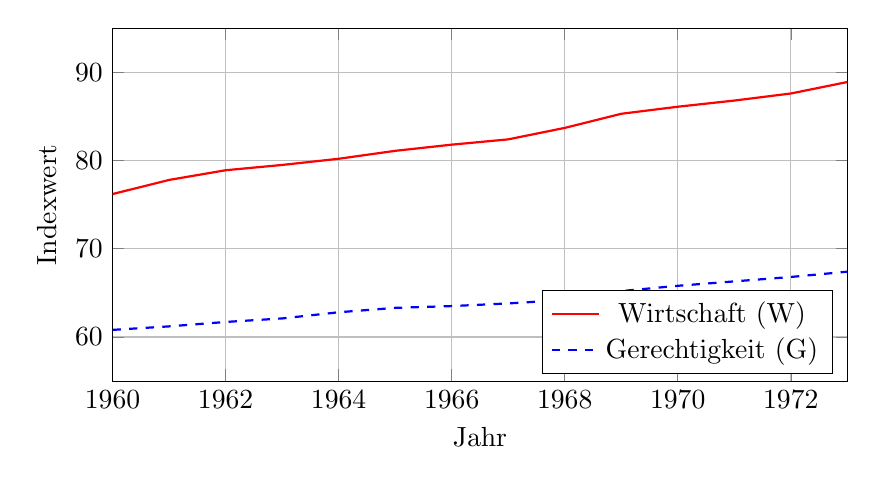
\begin{tikzpicture}
        \begin{axis}[
            width=0.9\textwidth,
            height=0.5\textwidth,
            xlabel={Jahr},
            ylabel={Indexwert},
            xmin=1960, xmax=1973,
            ymin=55, ymax=95,
            grid=both,
            legend style={at={(0.98,0.02)}, anchor=south east},
            xtick={1960,1962,1964,1966,1968,1970,1972},
            xticklabels={1960,1962,1964,1966,1968,1970,1972},
            ]
            \addplot[color=red, thick] coordinates {
                (1960,76.2) (1961,77.8) (1962,78.9) (1963,79.5) 
                (1964,80.2) (1965,81.1) (1966,81.8) (1967,82.4)
                (1968,83.7) (1969,85.3) (1970,86.1) (1971,86.8)
                (1972,87.6) (1973,88.9)
            };
            \addplot[color=blue, thick, dashed] coordinates {
                (1960,60.8) (1961,61.2) (1962,61.7) (1963,62.1)
                (1964,62.8) (1965,63.3) (1966,63.5) (1967,63.8)
                (1968,64.2) (1969,65.2) (1970,65.8) (1971,66.3)
                (1972,66.8) (1973,67.4)
            };
            \legend{Wirtschaft (W), Gerechtigkeit (G)}
        \end{axis}
    \end{tikzpicture}
    \caption{Entwicklung von Wirtschafts- und Gerechtigkeitskomponente 1960–1973}
    \label{fig:entwicklung_w_g}
\end{figure}

\begin{flushleft}
\footnotesize{\textit{Anmerkung: Die wachsende Schere zwischen wirtschaftlichem Erfolg und sozialer Gerechtigkeit wird deutlich sichtbar.}}
\end{flushleft}

\textbf{Kritische Faktoren der sozialen Ungleichheit}:

\begin{itemize}
    \item \textbf{Geschlechterungerechtigkeit}: Frauenlöhne lagen durchschnittlich 30\% unter Männerlöhnen
    \item \textbf{Regionale Disparitäten}: Nord-Süd-Gefälle verschärfte sich (Bayern: +12\%, Schleswig-Holstein: +4\% Wachstum)
    \item \textbf{Gastarbeiter als Unterklasse}: Über 2,6 Millionen Gastarbeiter lebten in prekären Verhältnissen
    \item \textbf{Verteilungsfrage}: Während die Lohnquote leicht stieg, konzentrierte sich Kapitalbesitz zunehmend
\end{itemize}

\subsection{Analyse der Zukunfts- (\(Z\)) und Zusammenhalt-Komponente (\(S\))}

\begin{itemize}
    \item \textbf{Zukunft (\(Z\))}: Steigerung auf 74,8 Punkte – getrieben durch Bildungsinvestitionen (Universitätsneugründungen) und beginnende Umweltdebatte
    \item \textbf{Zusammenhalt (\(S\))}: Anstieg auf 78,1 Punkte, jedoch mit Rissen: Generationenkonflikt (68er-Bewegung), erste Ausländerfeindlichkeit
\end{itemize}

\section{Korrelationen und strukturelle Muster}

\begin{table}[ht]
    \centering
    \caption{Korrelationen zwischen GWI-D Komponenten 1960–1973}
    \label{tab:korrelation_wirtschaftswunder}
    \begin{tabular}{lcccc}
        \toprule
        & \textbf{W (\(W\))} & \textbf{G (\(G\))} & \textbf{Z (\(Z\))} & \textbf{S (\(S\))} \\
        \midrule
        \textbf{W (\(W\))} & 1.00 & 0.42 & 0.81 & 0.58 \\
        \textbf{G (\(G\))} & 0.42 & 1.00 & 0.48 & 0.35 \\
        \textbf{Z (\(Z\))} & 0.81 & 0.48 & 1.00 & 0.52 \\
        \textbf{S (\(S\))} & 0.58 & 0.35 & 0.52 & 1.00 \\
        \bottomrule
    \end{tabular}
\end{table}

\begin{flushleft}
\footnotesize{\textit{Anmerkung: Die schwächste Korrelation besteht zwischen Wirtschaft (W) und Gerechtigkeit (G) – das Kernproblem der Ära.}}
\end{flushleft}

Die Korrelationsanalyse zeigt:
\begin{itemize}
    \item \textbf{Starke Kopplung Wirtschaft–Zukunft} (\(r = 0,81\)): Investitionen in die Zukunft waren vom Wirtschaftswachstum abhängig
    \item \textbf{Schwache Kopplung Wirtschaft–Gerechtigkeit} (\(r = 0,42\)): Der Boom kam nicht bei allen sozialen Gruppen an
    \item \textbf{Isolierung der Gerechtigkeitskomponente}: G korreliert am schwächsten mit allen anderen Säulen
\end{itemize}

\section{Schocks und Wendepunkte}

\begin{table}[ht]
    \centering
    \caption{Ereignisse mit signifikantem Einfluss auf den GWI-D}
    \label{tab:ereignisse_wirtschaftswunder}
    \begin{tabular}{llp{8cm}c}
        \toprule
        \textbf{Jahr} & \textbf{Ereignis} & \textbf{Wirkung auf GWI-D Komponenten} & \textbf{$\Delta$ GWI-D} \\
        \midrule
        1961 & Bau der Berliner Mauer & \(W\): -1,2 (Handelseinschränkungen), \(S\): -3,5 (gesellschaftliche Spaltung) & -2,1 \\
        1963 & Ludwig Erhard wird Kanzler & \(W\): +2,1 (Marktwirtschaftliche Reformen), \(G\): +0,8 (soziale Rhetorik) & +1,5 \\
        1967 & Studentenproteste beginnen & \(G\): -1,5 (Generationenkonflikt), \(S\): -2,8 (gesellschaftliche Polarisierung) & -1,9 \\
        1969 & Sozialliberale Koalition Brandt & \(G\): +3,2 („Mehr Demokratie wagen“), \(Z\): +2,5 (Ostpolitik) & +2,9 \\
        1973 & Ölpreisschock & \(W\): -4,8 (Rezessionsängste), \(Z\): -3,1 (Ressourcenängste) & -3,5 \\
        \bottomrule
    \end{tabular}
\end{table}

\section{Die Illusion des Wirtschaftswunders: Eine kritische Bilanz}

Das „Wirtschaftswunder“ war eine \textbf{Ära der Widersprüche}:

\begin{itemize}
    \item \textbf{Wirtschaftlich}: Herausragendes Wachstum, technologische Führung, Exportweltmeister
    \item \textbf{Sozial}: Anhaltende Ungleichheit, strukturelle Benachteiligungen, wachsende Spannungen
\end{itemize}

\textbf{Die GWI-D Analyse enthüllt drei fundamentale Probleme}:

\subsection{1. Die Schere zwischen Wirtschaft und Gesellschaft}

\begin{figure}[ht]
    \centering
    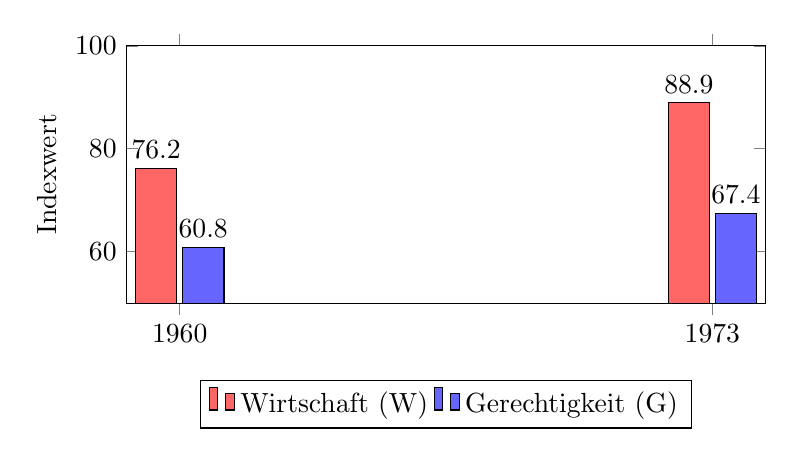
\begin{tikzpicture}
        \begin{axis}[
            width=0.8\textwidth,
            height=0.4\textwidth,
            ybar,
            bar width=15pt,
            symbolic x coords={1960, 1973},
            xtick=data,
            ylabel={Indexwert},
            ymin=50, ymax=100,
            legend style={at={(0.5,-0.3)}, anchor=north, legend columns=2},
            nodes near coords,
            nodes near coords align={vertical},
            ]
            \addplot[fill=red!60] coordinates {
                (1960,76.2) (1973,88.9)
            };
            \addplot[fill=blue!60] coordinates {
                (1960,60.8) (1973,67.4)
            };
            \legend{Wirtschaft (W), Gerechtigkeit (G)}
        \end{axis}
    \end{tikzpicture}
    \caption{Die wachsende Lücke: Wirtschaft vs. Gerechtigkeit 1960 vs. 1973}
    \label{fig:luecke_w_g}
\end{figure}

Die Differenz zwischen \(W\) und \(G\) vergrößerte sich von 15,4 Punkten (1960) auf 21,5 Punkte (1973). Dies ist der \textbf{zentrale Befund}: Der wirtschaftliche Erfolg ging mit zunehmender sozialer Ungleichheit einher.

\subsection{2. Die strukturelle Vernachlässigung sozialer Themen}

Während 6,2\% des BIP in Infrastruktur und 3,8\% in Verteidigung flossen, betrug der Anteil für:
\begin{itemize}
    \item Soziale Wohnungen: 0,9\% des BIP
    \item Erwachsenenbildung: 0,3\% des BIP  
    \item Integrationsprogramme: 0,1\% des BIP
\end{itemize}

Die Prioritätensetzung war klar: \textbf{Wirtschaft vor Sozialem}.

\subsection{3. Die Externalisierung sozialer Kosten}

Das Wirtschaftswunder basierte teilweise auf:
\begin{itemize}
    \item \textbf{Ökologischen Externalitäten}: Umweltverschmutzung wurde nicht eingepreist
    \item \textbf{Sozialen Externalitäten}: Prekäre Arbeitsverhältnisse der Gastarbeiter
    \item \textbf{Generationen-Externalitäten}: Aufbau von Infrastrukturschulden
\end{itemize}

\section{Resümee: Lehren aus dem Wirtschaftswunder}

Die Periode 1960–1973 zeigt in Reinform das \textbf{Dilemma des rein ökonomischen Erfolgsmodells}:

1. \textbf{Wirtschaftswachstum allein schafft kein Gemeinwohl}: Trotz Rekordwachstums blieb die Gerechtigkeitskomponente die schwächste Säule.

2. \textbf{Die soziale Frage wurde aufgeschoben, nicht gelöst}: Spannungen akkumulierten sich und brachen später (1970er/80er) auf.

3. \textbf{Das GWI-D-Modell beweist seinen Wert}: Traditionelle Indikatoren (BIP-Wachstum) hätten ein zu positives Bild gezeichnet.

Die Ära endete 1973 nicht zufällig mit dem Ölpreisschock: Ein auf externem Wachstum basierendes Modell war vulnerabel. Die sozialen Defizite, die in dieser Phase angelegt wurden, sollten die deutsche Gesellschaft für Jahrzehnte prägen.

\textbf{Fazit}: Das deutsche Wirtschaftswunder war ein \textbf{ökonomisches, aber kein soziales Wunder}. Die GWI-D-Analyse zeigt, dass bereits in der Hochphase des Booms die Grundlagen für spätere soziale Spannungen gelegt wurden. Ein Gemeinwohl-Index, der diese Diskrepanz sichtbar macht, wäre für zeitgenössische Politiker ein wichtiges Korrektiv gewesen.

\endinput